\documentclass{ltjsarticle}

\usepackage{graphicx}
\usepackage{here}
\usepackage{listings}
\usepackage{xcolor} 
\graphicspath{{../../public/img/}}

% \lstset{
%   language=Python, 
%   backgroundcolor=\color{gray!10}, 
%   basicstyle=\ttfamily, 
%   breaklines=true, 
%   commentstyle=\color{red}, 
%   frame=single, 
%   numbers=left, 
%   numberstyle=\tiny, 
%   showstringspaces=false, 
%   keywordstyle=\color{red}, 
%   stringstyle=\color{blue}, 
%   tabsize=2
% }
\lstset{
  language=Python,
  backgroundcolor=\color{black!85},
  basicstyle=\fontfamily{ttfamily}\selectfont\color{white},
  breaklines=true,
  commentstyle=\color{green!50!black},
  frame=none,
  framexleftmargin=10mm,
  framexrightmargin=10mm,
  numbers=left,
  numberstyle=\tiny\color{gray},
  showstringspaces=false,
  keywordstyle=\color{blue!40!cyan},
  stringstyle=\color{orange},
  tabsize=2,
  morekeywords={import, from, class, def, for, while, if, is, in, elif, else, not, and, or, print, break, continue, return, True, False, None, assert, async, await, as},
}

\title{深層学習 第一回}
\author{37246392 豊田圭将}
\date{2024/04/11}

\begin{document}

\maketitle

\section{やったこと・動かしたものの概要}

\begin{enumerate}
  \item OpenAI APIを使ってキーワードから名詞句を作成
  \item Stable Diffusionを使って名詞句から画像生成
  \item CLIPを使って、2の画像に1のキーワードが含まれている確率をそれぞれ計算
\end{enumerate}

\section{具体的な手続き}

\subsection{OpenAI APIを使ってキーワードから名詞句を作成}
\begin{itemize}
  \item キーワード: rabbit, moon, football
  \item 名詞句: a rabbit playing football on the moon
\end{itemize}

\subsection{Stable Diffusionを使って名詞句から画像生成}
\begin{itemize}
  \item プロンプト: a rabbit playing football on the moon
  \item 生成された画像: \\

        \begin{figure}[H]
          \centering
          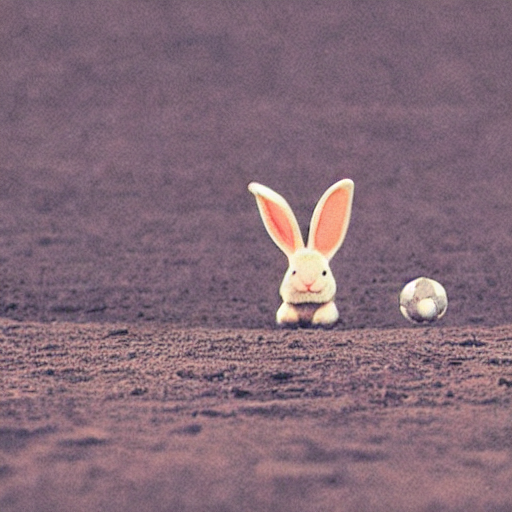
\includegraphics[width=6cm]{a_rabbit_playing_football_on_the_moon.png}
        \end{figure}
\end{itemize}

\subsection{CLIPを使って、2の画像に1のキーワードが含まれている確率をそれぞれ計算}
\begin{itemize}
  \item rabbit: 0.937
  \item moon: 0.0047
  \item football: 0.058
\end{itemize}

\subsection{ソースコード}
\lstinputlisting{../../src/1_20240411/main.py}

\section{わかったこと・わからなかったこと}

Stable Diffusionを始めて使用したが、非常に簡単に画像を生成できることがわかった。また、CLIPを使って画像に含まれるキーワードを推定したが、YOLOなどの物体検出と比べて精度が良いのかも試してみたい。

\end{document}